\documentclass[aspectratio=169]{beamer}
\usepackage{pgfpages}

\usepackage{datetime}
\newdateformat{mydate}{\twodigit{\THEDAY}/\twodigit{\THEMONTH}/\THEYEAR}

\usepackage[backend=biber, style=ieee]{biblatex}
\addbibresource{Bibliography.bib}
\renewcommand{\bibfont}{\tiny}

\usepackage{svg}
\usepackage{subcaption}
\usepackage{graphicx}
\usepackage{multicol}
\usepackage{algorithm}
\usepackage{algorithmic}
\usepackage{animate}
\usepackage{appendixnumberbeamer}
\usepackage{etoolbox}
\usepackage{adjustbox}
\usepackage{multimedia}

\usepackage[font=footnotesize]{caption}
\usepackage{color, colortbl}
\usepackage{multirow}

\usepackage[acronym]{glossaries}
\makenoidxglossaries
\input{acronym.tex}

\usetheme{Warsaw}
\setbeamertemplate{navigation symbols}{}

\setbeamertemplate{bibliography item}{\insertbiblabel}
\setbeamertemplate{blocks}[rounded][shadow=false]

\makeatletter
\pgfdeclareverticalshading[lower.bg,upper.bg]{bmb@transition}{200cm}{%
  color(0pt)=(lower.bg); color(2pt)=(lower.bg)
}
\makeatother

\definecolor{UniBEred}{RGB}{226, 0, 43}
\definecolor{UniBEblack}{RGB}{19, 17, 16}
\definecolor{Timaorange}{RGB}{224, 111, 83}
\setbeamercolor{structure}{fg=UniBEblack}
\setbeamercolor{frametitle}{bg=UniBEblack}
\setbeamercolor{frametitle right}{bg=UniBEblack}
\setbeamercolor{block title example}{use=Timaorange,fg=white,bg=Timaorange}
\newcommand{\highlightcell}[1]{\cellcolor{Timaorange}\textcolor{white}{#1}}
\setbeamertemplate{itemize item}{\scalebox{0.45}{$\blacksquare$}}
\setbeamertemplate{itemize subitem}{{$\circ$}}
\setbeamertemplate{enumerate item}{\roman{enumi}}
\AtBeginEnvironment{exampleblock}{
  \setbeamercolor{itemize item}{fg=Timaorange}
  \setbeamercolor{itemize subitem}{fg=Timaorange}
}
\newenvironment<>{boite1}[1]{%
  \setbeamercolor{block title}{use=UniBEred,fg=white,bg=UniBEred}%
  \setbeamercolor{block body}{bg=white}
  \setbeamercolor{itemize item}{fg=UniBEred}
  \setbeamercolor{itemize subitem}{fg=UniBEred}
  \begin{block}#2{\centering \textbf{#1}}}{\end{block}}

\newenvironment<>{boite}[1]{%
  \setbeamercolor{block title}{use=UniBEblack,fg=white,bg=UniBEblack}%
  \setbeamercolor{block body}{bg=white}
  \setbeamercolor{itemize item}{fg=UniBEblack}
  \setbeamercolor{itemize subitem}{fg=UniBEblack}
  \begin{block}#2{\centering \textbf{#1}}}{\end{block}}

% For a title slide to each section
\AtBeginSection[]{
  \setbeamercolor{structure}{fg=UniBEblack}
  \setbeamercolor{frametitle}{bg=UniBEblack}
  \setbeamercolor{frametitle right}{bg=UniBEblack}
  \begin{nonumberframe}{Table of contents}{\insertsection}
    \begin{columns}[t]
      \begin{column}{.5\textwidth}
          \centering
          \textbf{INTEGRATED CIRCUITS}
          \tableofcontents[currentsection,hideothersubsections,part={1}]
      \end{column}
      \begin{column}{.5\textwidth}
          \centering
          \textbf{ASYNCHRONOUS CIRCUITS}
          \tableofcontents[currentsection,hideothersubsections,part={2}]
      \end{column}
  \end{columns}
  \end{nonumberframe}
}


\setbeamertemplate{section in toc}[circle]
\setbeamertemplate{subsection in toc}[square]


\setbeamerfont{section number projected}{size=\large}
\setbeamercolor{section number projected}{bg=UniBEblack,fg=white}

% \AtBeginSubsection[]{
%   \begin{nonumberframe}
%   \vfill
%   \centering
%   \begin{beamercolorbox}[sep=8pt,center,shadow=true,rounded=true]{title}
%     \usebeamerfont{title}\insertsubsectionhead\par%
%   \end{beamercolorbox}
%   \vfill
%   \end{nonumberframe}
% }

\usepackage[footheight=1em]{beamerthemeboxes}

\setbeamercolor{footlinecolor}{bg=UniBEblack,fg=white}

\newenvironment{nonumberframe}{%
    \setbeamertemplate{footline}{%
    \leavevmode%
    \hbox{\begin{beamercolorbox}[wd=\paperwidth,ht=2.5ex,dp=1.125ex,leftskip=.3cm,rightskip=.3cm]{footlinecolor}%
    \inserttitle \ - \insertshortauthor
    \end{beamercolorbox}%
    }%
    \vskip 0pt%
    }
    \begin{frame}[noframenumbering] %Remove the noframenumbering option if you want the counter to be increased on a frame that is not numbered.
    }{%
    \end{frame}
}

\makeatother
\setbeamertemplate{footline}
{%
  \leavevmode%
  \hbox{\begin{beamercolorbox}[wd=.8\paperwidth,ht=2.5ex,dp=1.125ex,leftskip=.3cm,rightskip=.3cm]{footlinecolor}%
  \inserttitle ~- \mydate\insertdate ~- \insertshortauthor
  \end{beamercolorbox}%
  \begin{beamercolorbox}[wd=.2\paperwidth,ht=2.5ex,dp=1.125ex,leftskip=.3cm,rightskip=.3cm plus1fil]{footlinecolor}%
    \hfill\insertframenumber/\inserttotalframenumber
  \end{beamercolorbox}
  }%
  \vskip 0pt%
}
\makeatletter

% \addfootboxtemplate{\color{UniBEblack}}{\color{white}\hspace*{0.3cm} Reunion \ \insertdate \ - \insertshortauthor}
% \addfootboxtemplate[.2\paperwidth]{\color{UniBEblack}}{\color{white}
%      \hfill\insertframenumber/\inserttotalframenumber\hspace*{2em}\null}

\title{Asynchronous Integrated Circuits}
\subtitle{An Introduction}
\author[X. Lesage]{Xavier Lesage}
\date{\today}

\begin{document}

%\input{tikz_config.tex}

% \begin{nonumberframe}
%     \titlepage
% \end{nonumberframe}

\begin{nonumberframe}
  \begin{beamercolorbox}[sep=8pt,center,rounded=true]{title}
    \usebeamerfont{title}\inserttitle\par%
    \usebeamerfont{subtitle}\insertsubtitle
  \end{beamercolorbox}%

  \vspace{1cm}

  \begin{columns}[c]
    \begin{column}{0.33\textwidth}
      \begin{figure}
        \centering
        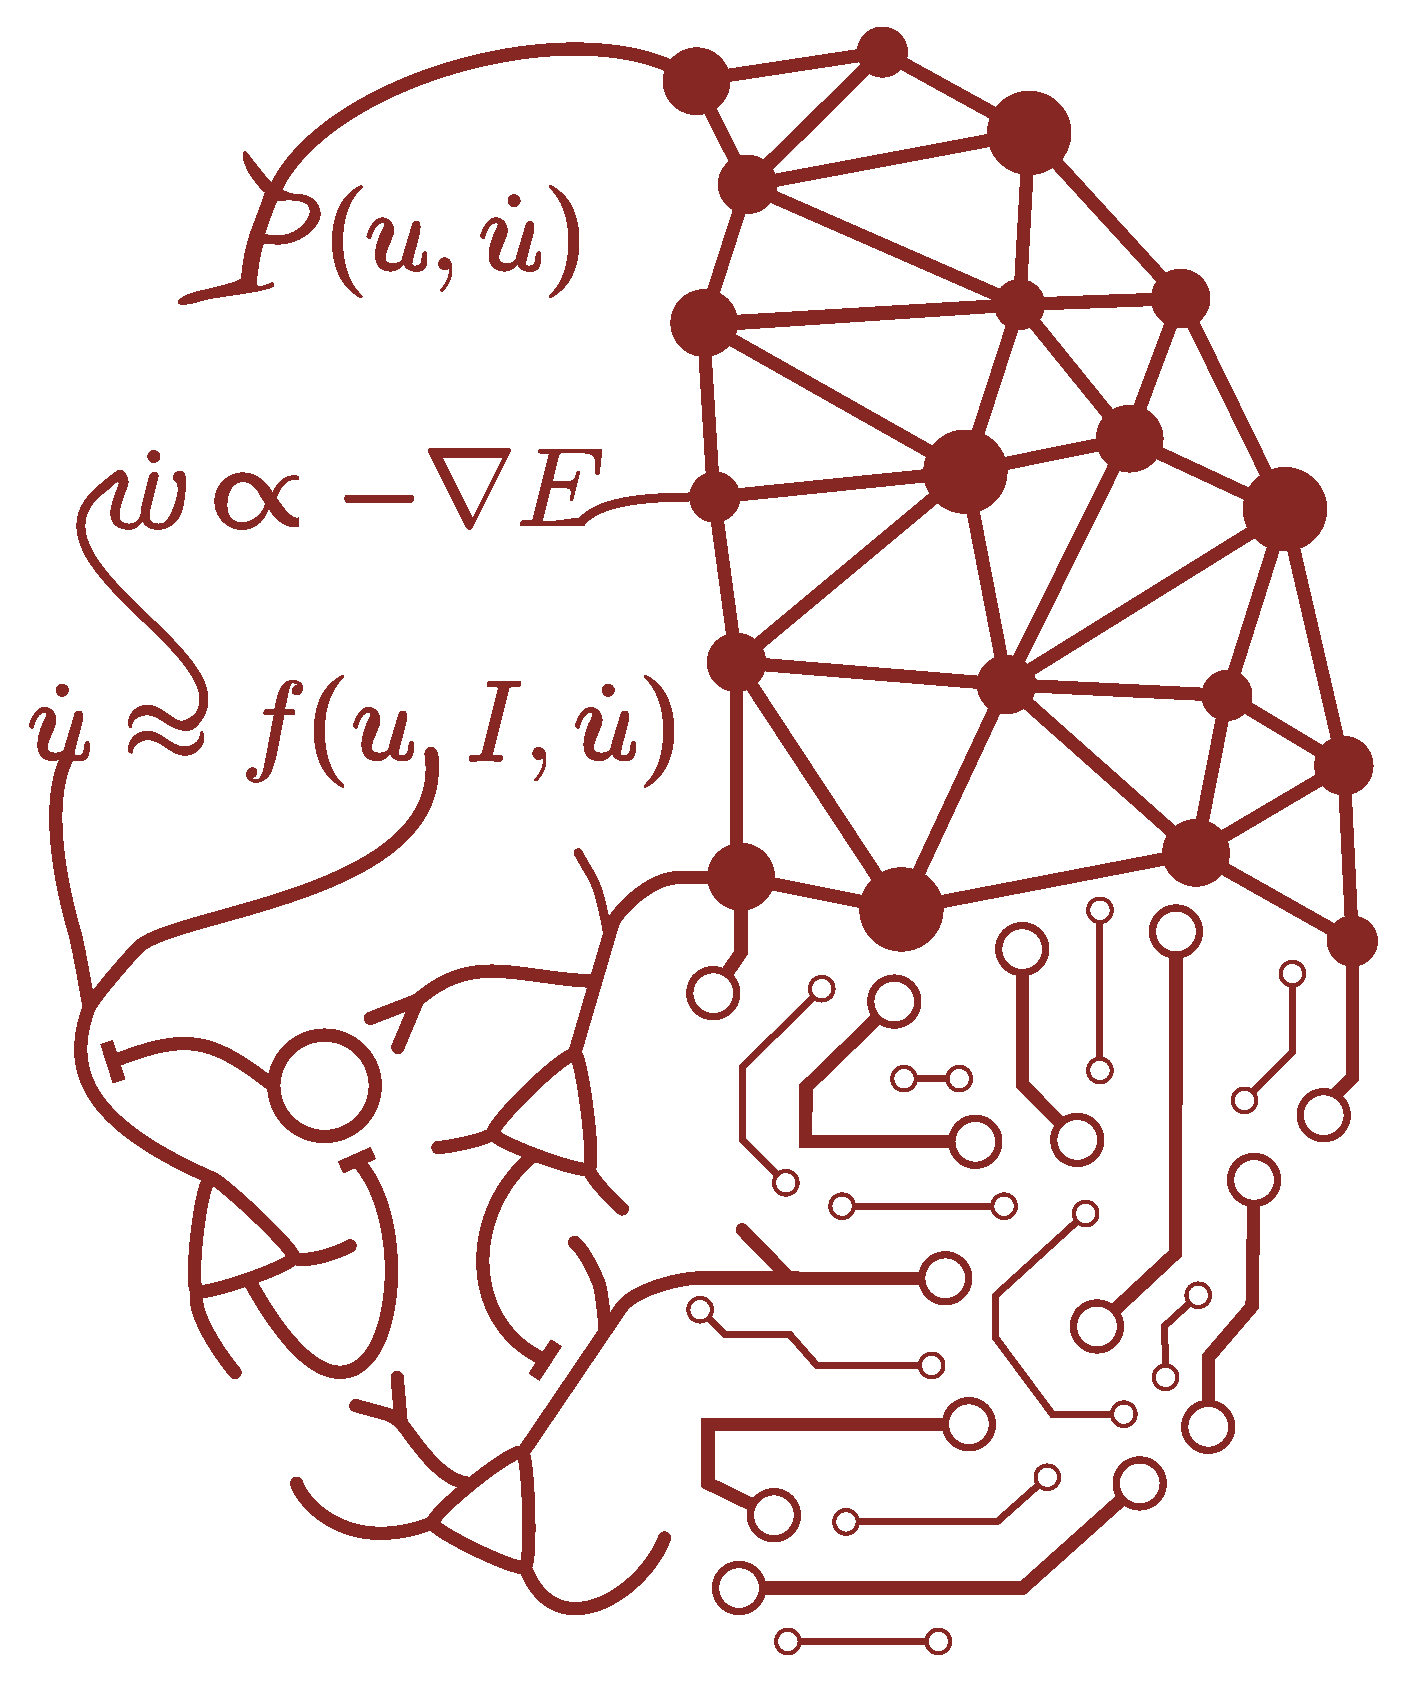
\includegraphics[width= .4\textwidth]{Logos/Logo_red.png}
    \end{figure}
      % \vspace{1cm}
    \begin{figure}
        \centering
        
\includegraphics[width= .4\textwidth]{Logos/Unibe_White_logo.png}
    \end{figure}
    \end{column}

    \begin{column}{0.65\textwidth}
      \usebeamerfont{author}\insertauthor\par
      \vspace{0.3cm}
      \usebeamerfont{institute}\insertinstitute\par
      \usebeamerfont{date}\insertdate
    \end{column}
  \end{columns}
\end{nonumberframe}


\part{Integrated Circuits}
\begin{nonumberframe}
    \vfill
    \centering
    \begin{beamercolorbox}[sep=8pt,center,shadow=false,rounded=true]{title}
    \usebeamerfont{title}Part I - INTEGRATED CIRCUITS\par%
    \usebeamerfont{subtitle} GUT meeting 13/01/2026
    \end{beamercolorbox}
    \vfill
\end{nonumberframe}

\section{Abstractions}
\subsection{Layers}
\begin{frame}{\insertsubsection}{\insertsection}
   % One or more splide to present the abstractions layer
   % System, Data Flow (Pipelines, Algorithm), Modules, Netlist Gate-level, Physical design, Waffer
    \begin{figure}
        \centering
        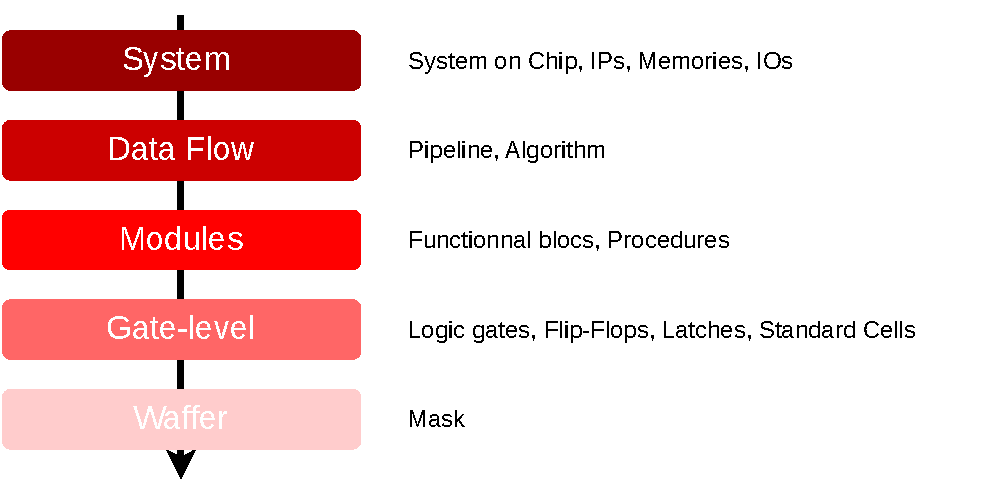
\includegraphics[width=\linewidth]{Figures/abstractions.pdf}
    \end{figure}
\end{frame}

\subsection{Combinational Logic}
\begin{frame}{Boolean Algebra}{\insertsection ~- \insertsubsection}
    \begin{columns}
        \column{0.65\textwidth}
        \begin{align}
            S &= \bar{A} \bar{B} {C_{in}} + \bar{A} {B} \bar{C_{in}} + {A} \bar{B} \bar{C_{in}} + {A} {B} {C_{in}} \label{eq:dnf_s}\\
            S &= A \oplus B \oplus {C_{in}} \\
            C_{out} &= \bar{A} {B} {C_{in}} + {A} \bar{B} {C_{in}} + A B \bar{C_{in}} + A B {C_{in}} \label{eq:dnf_cout}\\
            C_{out} &= A B + {C_{in}} ( A \oplus B)
        \end{align}

        \begin{boite1}{Note}
            \begin{itemize}
                \item (\ref{eq:dnf_s}) and (\ref{eq:dnf_cout}) are in Disjunctive Normal Form (DNF)
            \end{itemize}
        \end{boite1}

        \column{0.35\textwidth}
        \begin{table}[]
        \begin{tabular}{|ccc|cc|}
        \hline
        \multicolumn{3}{|c|}{Input}                              & \multicolumn{2}{c|}{Output}     \\ \hline
        \multicolumn{1}{|c|}{$A$} & \multicolumn{1}{c|}{$B$} & $C_{in}$ & \multicolumn{1}{c|}{$S$} & $C_{out}$ \\ \hline \hline
        0                       & 0                      & 0     & 0                      & 0      \\
        0                       & 0                      & 1     & 1                      & 0      \\
        0                       & 1                      & 0     & 1                      & 0      \\
        0                       & 1                      & 1     & 0                      & 1      \\
        1                       & 0                      & 0     & 1                      & 0      \\
        1                       & 0                      & 1     & 0                      & 1      \\
        1                       & 1                      & 0     & 0                      & 1      \\
        1                       & 1                      & 1     & 1                      & 1      \\ \hline
        \end{tabular}
        \end{table}
    \end{columns}
\end{frame}
\begin{frame}{Logic Gates}{\insertsection ~- \insertsubsection}
    \begin{figure}
        \centering
        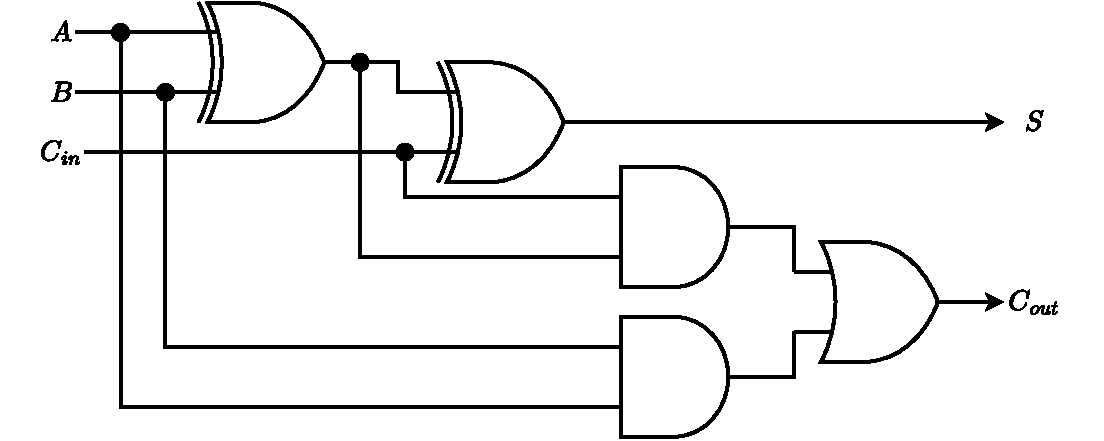
\includegraphics[width=\linewidth]{Figures/FA_gates.pdf}
    \end{figure}
\end{frame}
\begin{frame}{Transitor Implementation}{\insertsection ~- \insertsubsection}
    \begin{columns}[T]
        \column{0.3\textwidth}
            \begin{figure}
                \centering
                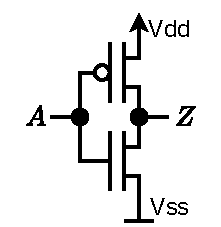
\includegraphics[scale=0.9]{Figures/trans_inverter.pdf}
            \end{figure}
            \vspace{1.2cm}
            \centering
            Inverter gate CMOS
        \column{0.3\textwidth}
            \begin{figure}
                \centering
                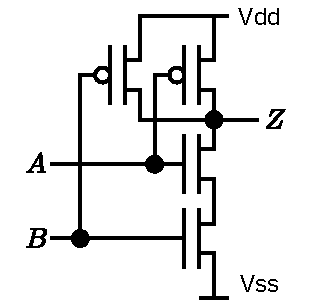
\includegraphics[scale=0.9]{Figures/trans_nand.pdf}
            \end{figure}
            \vfill
            \centering
            NAND gate CMOS
        \column{0.3\textwidth}
            \begin{figure}
                \centering
                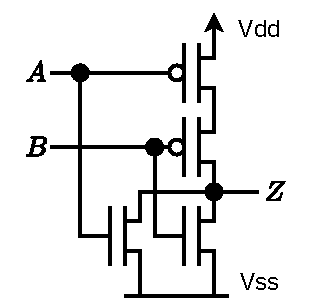
\includegraphics[scale=0.9]{Figures/trans_nor.pdf}
            \end{figure}
            \vfill
            \centering
            NOR gate CMOS
    \end{columns}
\end{frame}
\begin{frame}{Mask}{\insertsection ~- \insertsubsection}
    \begin{columns}
        \column{0.4\textwidth}
            \begin{figure}
                \centering
                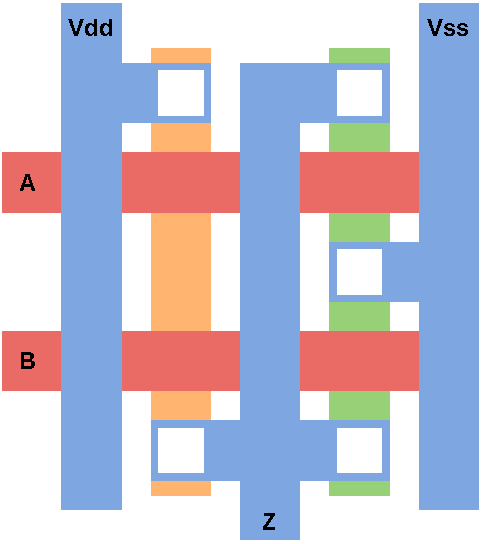
\includegraphics[scale=0.65]{Figures/mask_nor.pdf}
            \end{figure}
        \column{0.6\textwidth}
            \begin{columns}
                \column{0.2\columnwidth}
                    \begin{figure}
                        \centering
                        
\includegraphics[scale=0.65]{Figures/mask_metal.pdf}
                    \end{figure}
                \column{0.7\columnwidth}
                    \vspace{-0.35cm}
                    Metal
            \end{columns}
            \begin{columns}
                \column{0.2\columnwidth}
                    \begin{figure}
                        \centering
                        
\includegraphics[scale=0.65]{Figures/mask_poly.pdf}
                    \end{figure}
                \column{0.7\columnwidth}
                    \vspace{-0.35cm}
                    Gate (polysilicon)
            \end{columns}
                        \begin{columns}
                \column{0.2\columnwidth}
                    \begin{figure}
                        \centering
                        
\includegraphics[scale=0.65]{Figures/mask_diff_p.pdf}
                    \end{figure}
                \column{0.7\columnwidth}
                    \vspace{-0.35cm}
                    P diffusion
            \end{columns}
                        \begin{columns}
                \column{0.2\columnwidth}
                    \begin{figure}
                        \centering
                        
\includegraphics[scale=0.65]{Figures/mask_diff_n.pdf}
                    \end{figure}
                \column{0.7\columnwidth}
                    \vspace{-0.35cm}
                    N diffusion
            \end{columns}
    \end{columns}
\end{frame}


\section{Design Families}
\subsection{Overview}
\begin{frame}{\insertsubsection}{\insertsection}
   % Frame with Flexibility vs Performance Figure

    \begin{figure}
        \centering
        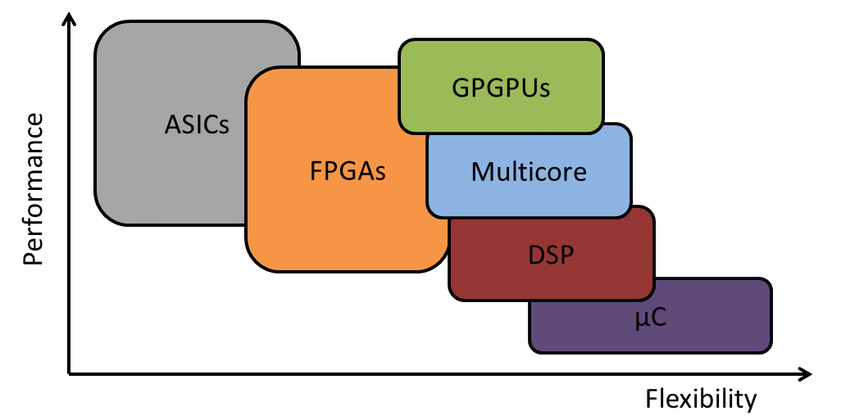
\includegraphics[width=.9\textwidth]{Figures/Performance-vs-Flexibility.png}
        \caption{Performance vs Flexibility \cite{article}}
    \end{figure}

\end{frame}

\subsection{Central Processing Unit}
\begin{frame}{Instruction Set Architecture}{\insertsection ~- \insertsubsection}
    % Present ISA and programs
    % Present SISD
    \begin{columns}
        \column{0.42\textwidth}
        \begin{itemize}
            \item Instruction Set Architecture (ISA)
            \item Single Instruction Single Data (SISD)
            \item Executes a program stored in memory
        \end{itemize}

        \column{0.6\textwidth}
        \begin{figure}
            \centering
            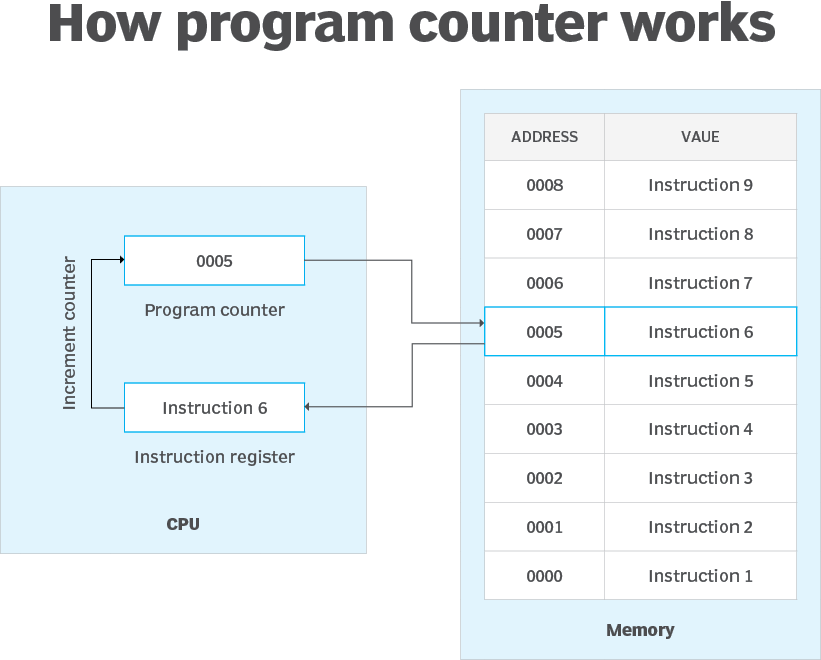
\includegraphics[width=.9\textwidth]{Figures/how_program_counter_works.png}
            \caption{Program \cite{noauthor_what_nodate}}
        \end{figure}
        % Figure
    \end{columns}
\end{frame}

\begin{frame}{Von Neumann \& Harvard Architecture}{\insertsection ~- \insertsubsection}
    % Compare the system view of Van Neumann and Harvard
    % Main Components (IO, Memory, Execution)
    \begin{columns}
        \column{0.49\textwidth}
        \begin{figure}
            \centering
            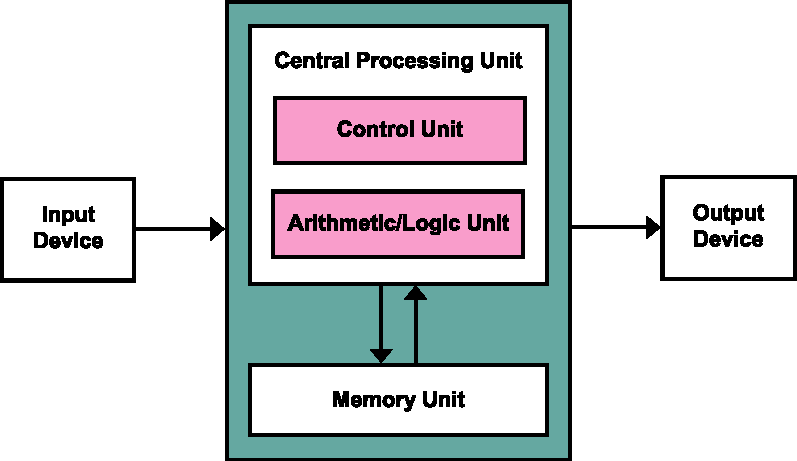
\includegraphics[width=\textwidth]{Figures/Von_Neumann_Architecture.pdf}
            \caption{Von Neumann Architecture \cite{noauthor_von_2025}}
        \end{figure}

        \column{0.49\textwidth}
        \begin{figure}
            \centering
            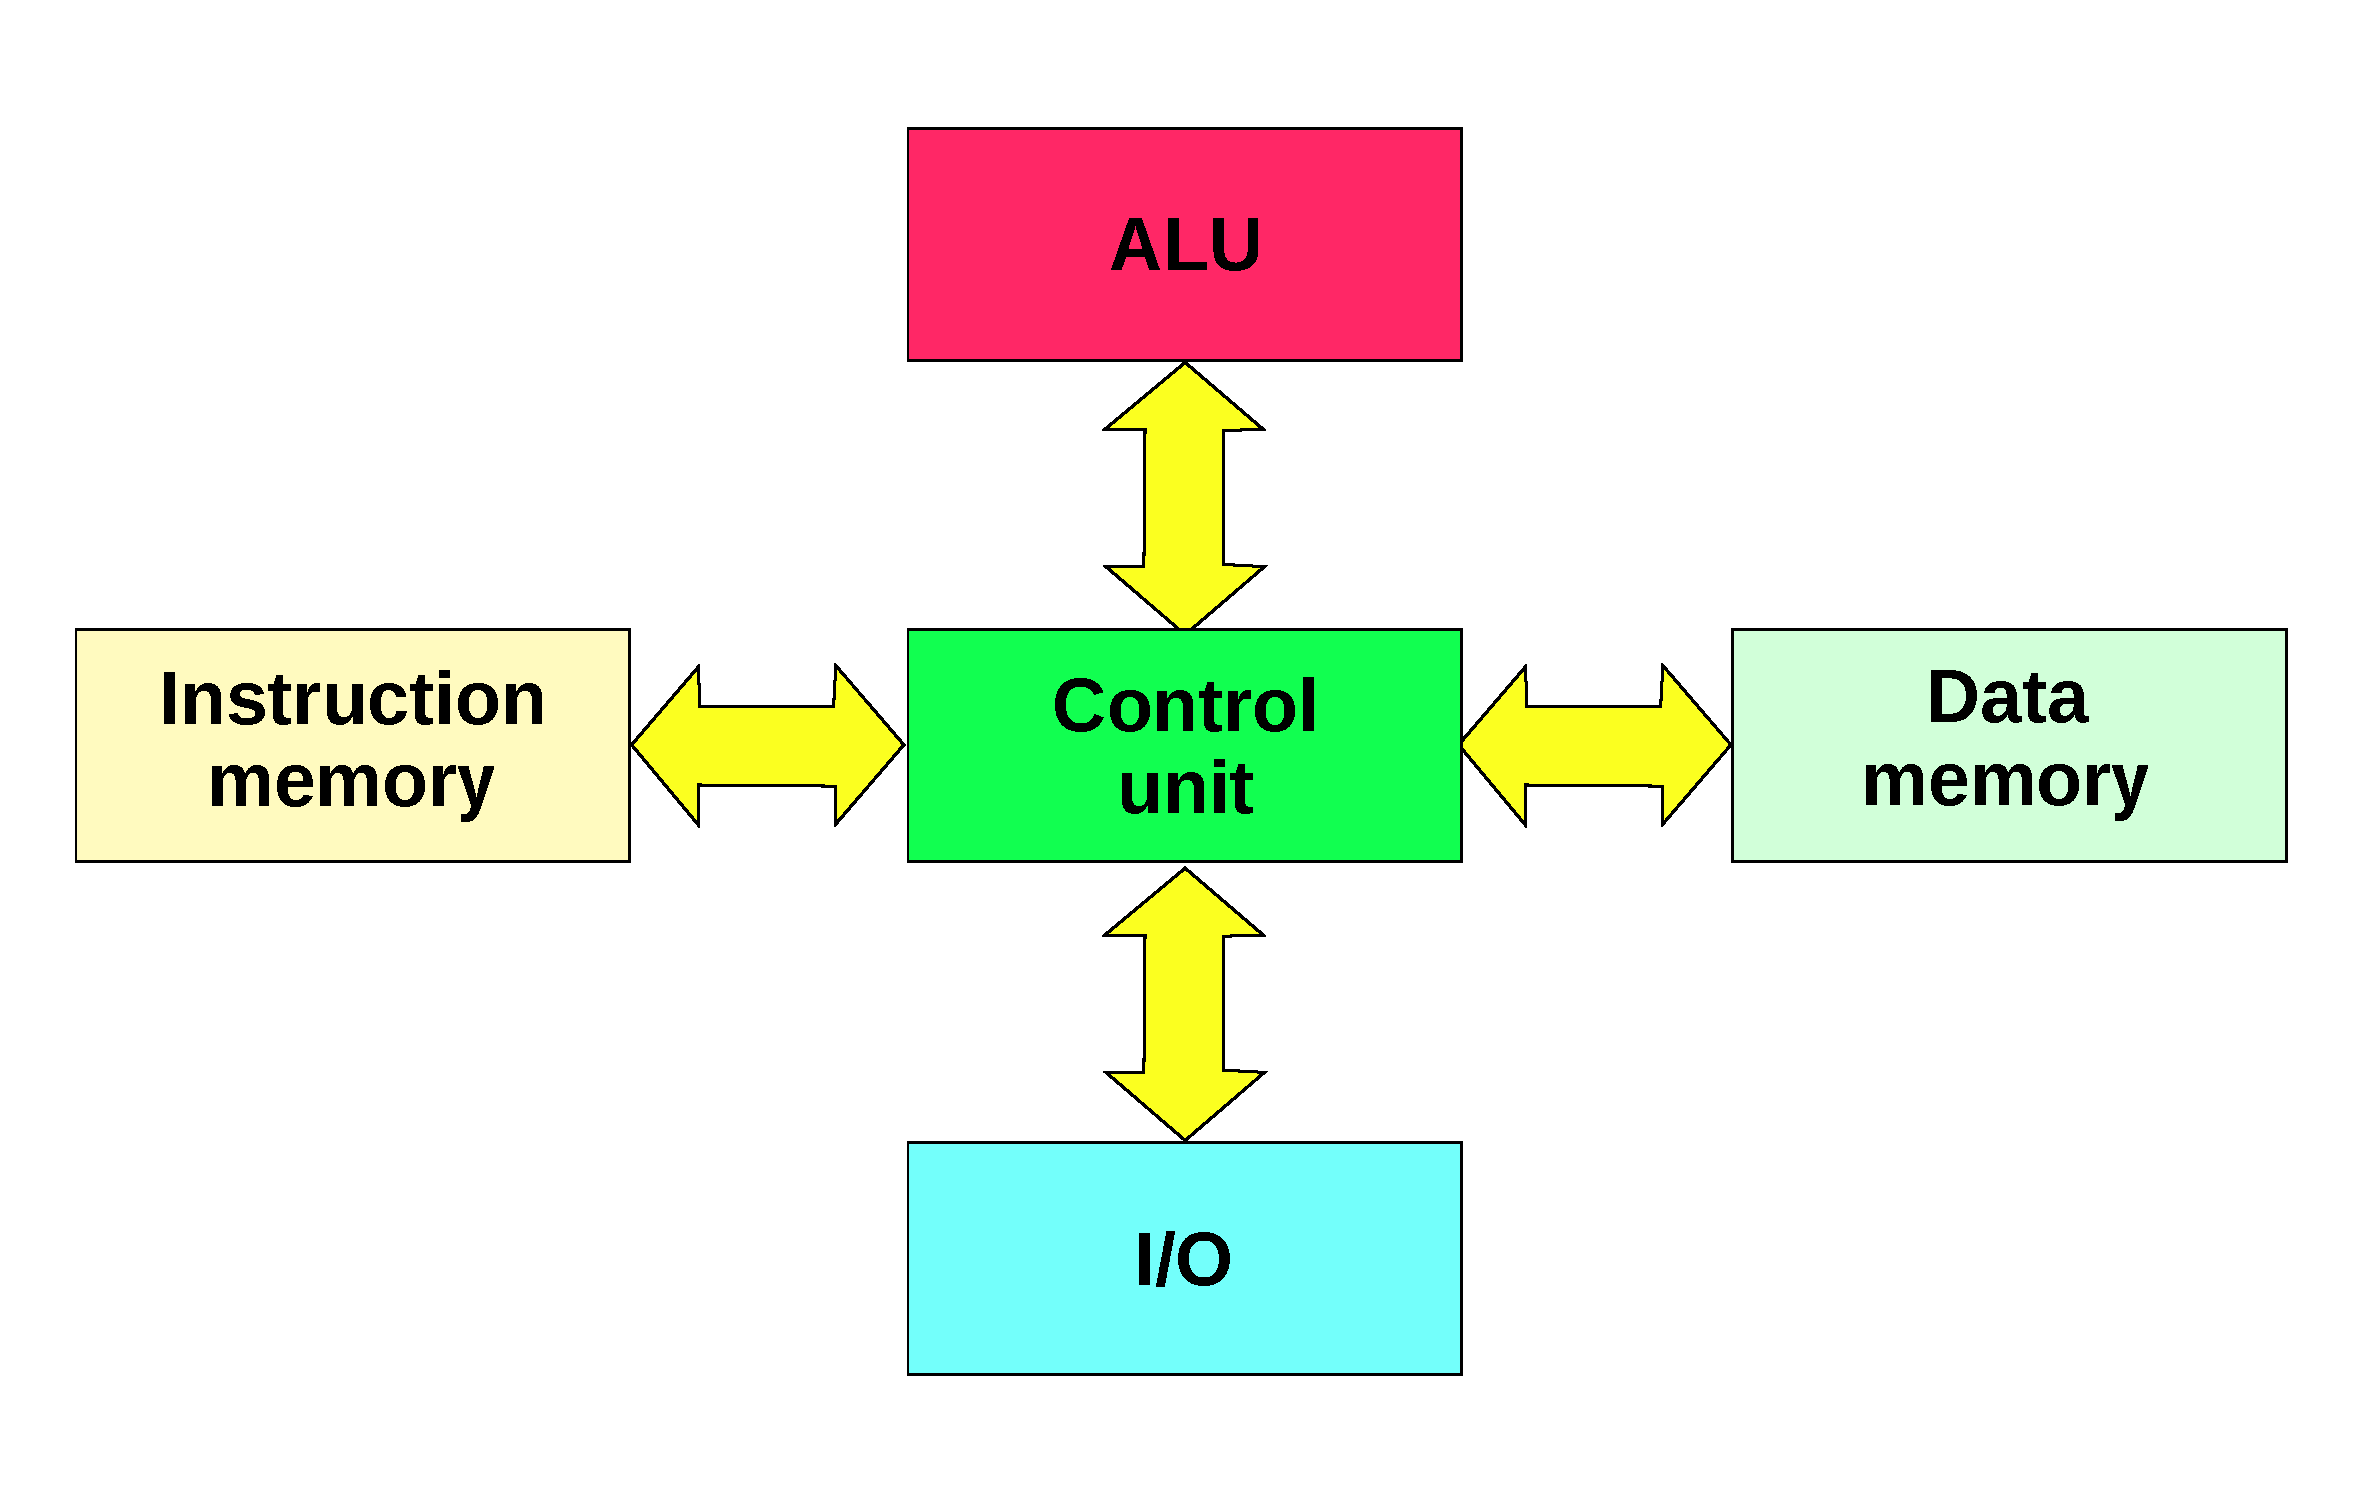
\includegraphics[width=\textwidth]{Figures/Harvard_architecture.pdf}
            \caption{Harvard Architecture \cite{noauthor_harvard_2025}}
        \end{figure}
    \end{columns}
\end{frame}

\begin{frame}{Execution Pipeline}{\insertsection ~- \insertsubsection}
    % Present the 5 stage execution pipeline
    \begin{columns}
        \column{0.4\textwidth}
        Stages :
        \begin{itemize}
            \item IF: Instruction Fetch
            \item ID: Instruction Decode
            \item EX: Execute
            \item MEM: Memory access
            \item WB: WriteBack
        \end{itemize}

        \column{0.6\textwidth}
        \begin{figure}
            \centering
            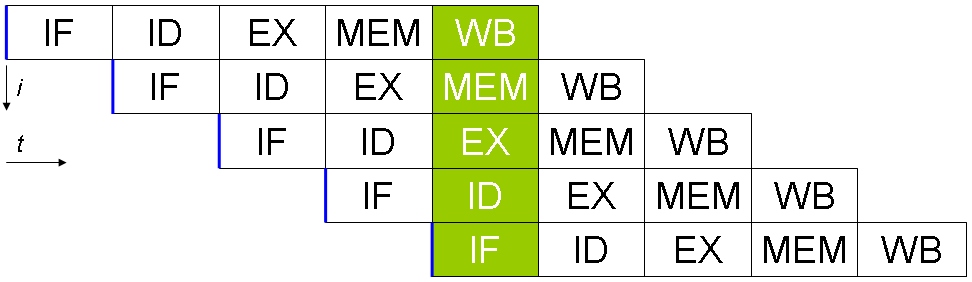
\includegraphics[width=\textwidth]{Figures/Fivestagespipeline.png}
            \caption{Five stage pipeline \cite{noauthor_classic_2025}}
        \end{figure}
    \end{columns}
\end{frame}

\subsection{Graphical Processing Unit}
\begin{frame}{Single Instruction Multiple Data}{\insertsection ~- \insertsubsection}
    % Present SIMD
    % Present vector computation
    \begin{columns}
        \column{0.49\textwidth}
        \begin{itemize}
            \item Single Instruction Multiple Data (SIMD)
            \item Vector operations
            \begin{itemize}
                \item e.g. scalar multiplication $a\vec{v}$
            \end{itemize}
        \end{itemize}

        \column{0.5\textwidth}
        \begin{figure}
            \centering
            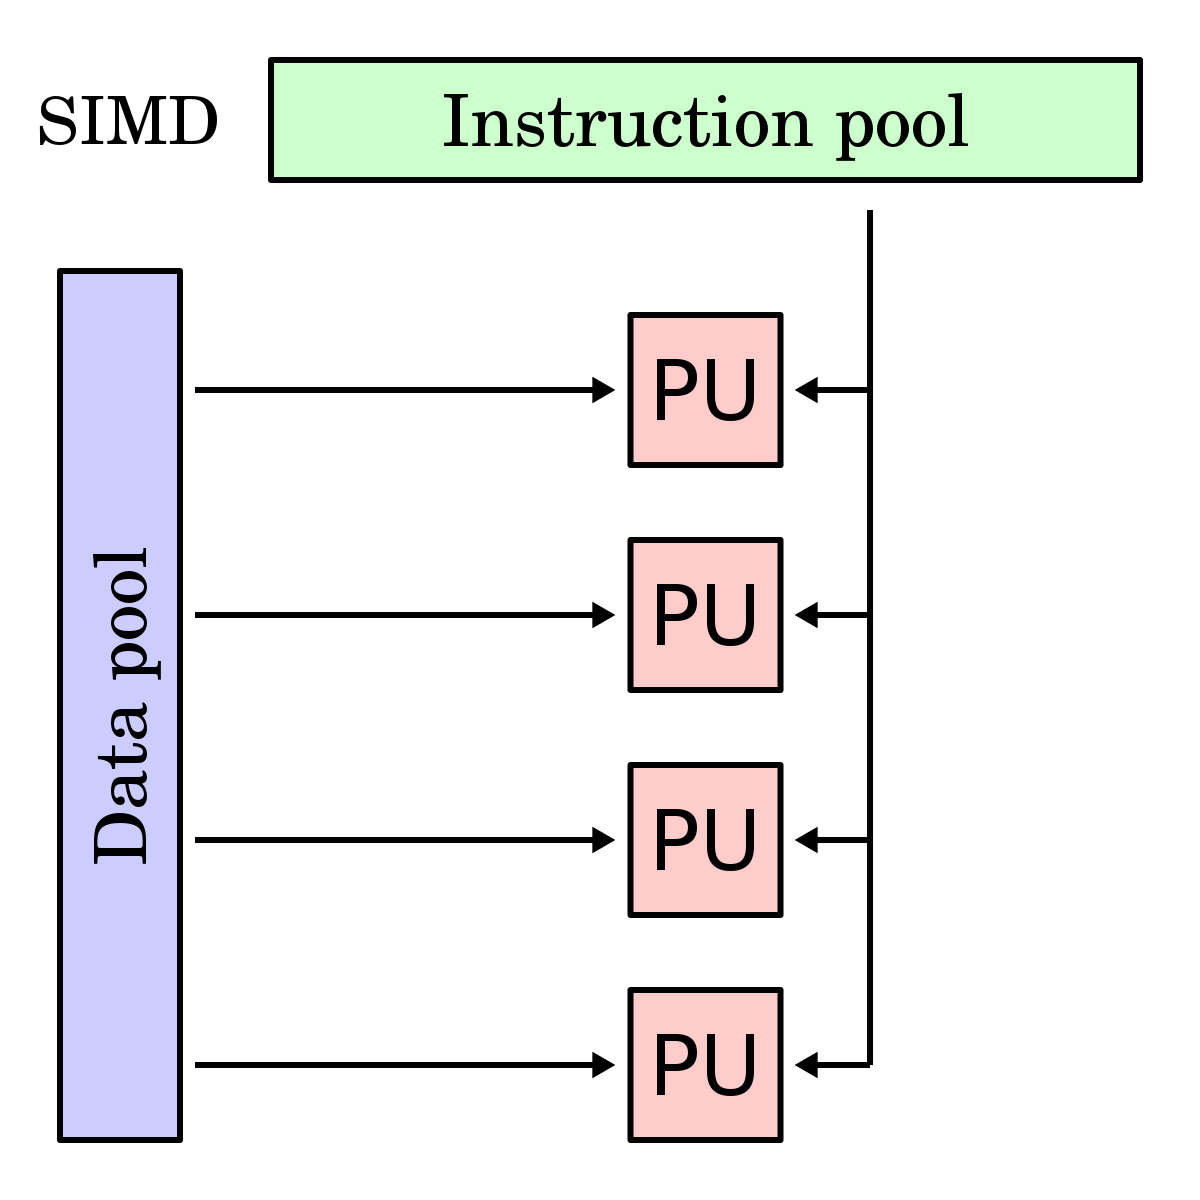
\includegraphics[width=.85\textwidth]{Figures/simd.png}
            \caption{Instruction to Processing Unit (PU) \cite{noauthor_simd_nodate}}
        \end{figure}
    \end{columns}
\end{frame}

\begin{frame}{Parallel vs Serial}{\insertsection ~- \insertsubsection}
    \centering
    Multiply ACcumulation (MAC) operation in dot product $\vec{a} \cdot \vec{b}$
    % Compare implementations in term of performance, area, latency etc
    % Present a MAC as an example ?
    \begin{columns}[T]
        \column{0.49\textwidth}
        \centering
        Serial:
        % \vspace{1.8cm}
        \begin{figure}
            \centering
            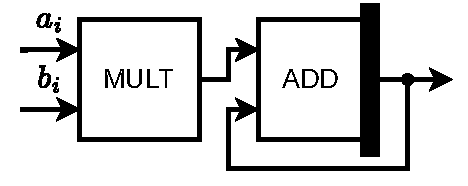
\includegraphics[scale=0.55]{Figures/serial.pdf}
        \end{figure}
        \begin{boite1}{Comparison}
            \begin{itemize}
                \item Size
                \item Power consumption
                \item Latency
            \end{itemize}
        \end{boite1}

        \column{0.49\textwidth}
        \centering
        Parallel:
        \begin{figure}
            \centering
            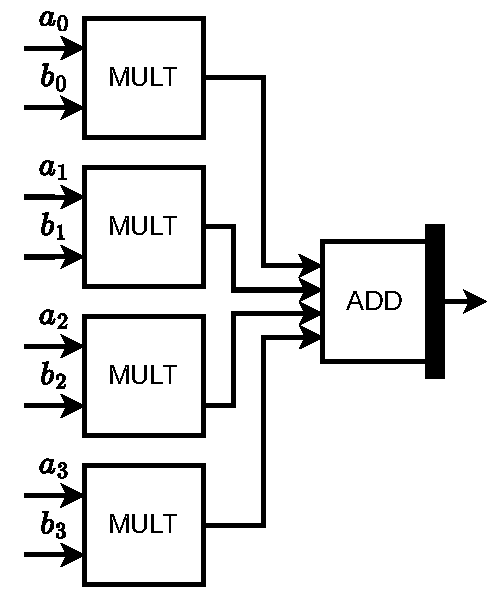
\includegraphics[scale=0.55]{Figures/parallel.pdf}
        \end{figure}
    \end{columns}
\end{frame}

\subsection{Field-Programmable Gate Array \cite{noauthor_what_2024}}
\begin{frame}{\insertsubsection}{\insertsection}
    % Present reconfigurable hardware
    % Present LUT architecture
    \begin{columns}[c]
        \column{0.49\textwidth}
        \centering
        % \vspace{1.8cm}
        \begin{figure}
            \centering
            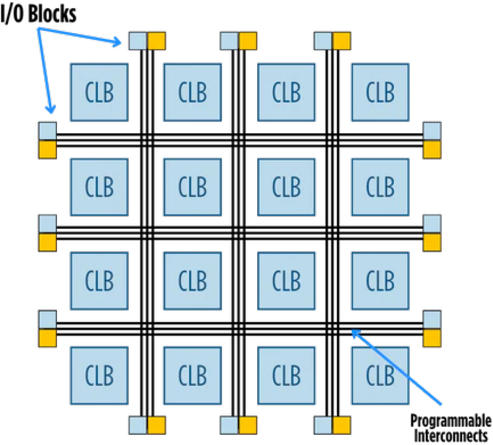
\includegraphics[width=\textwidth]{Figures/fpga_board.pdf}
        \end{figure}

        \column{0.49\textwidth}
        \centering
        \begin{figure}
            \centering
            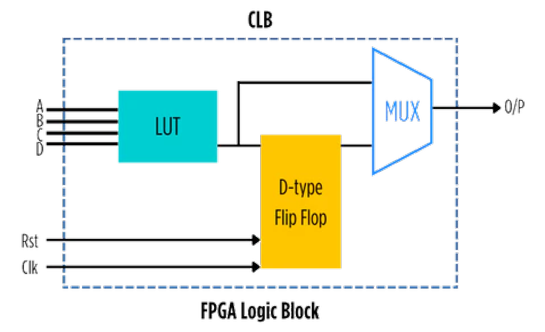
\includegraphics[width=\textwidth]{Figures/fpga_CLB.pdf}
        \end{figure}
    \end{columns}
\end{frame}

\subsection{System on Chip}
\begin{frame}{\insertsubsection}{\insertsection}
    % Present a computing platform with a bus, Peripheral bridge and memories
    \begin{figure}
        \centering
        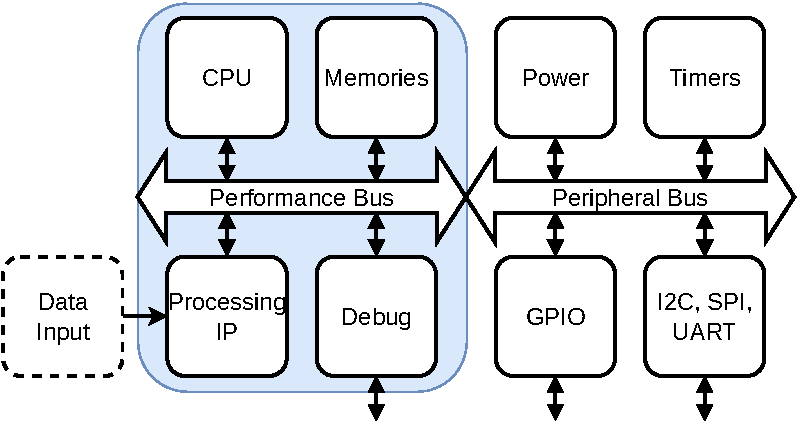
\includegraphics[width=.9\textwidth]{Figures/system_bus.pdf}
    \end{figure}
\end{frame}

% \subsection{Application-Specific Integrated Circuit \& IPs}
% \begin{frame}{\insertsubsection}{\insertsection}
%     % System on Chip with IPs
%     % Multi-abstraction level design
%     \begin{columns}[c]
%         \column{0.49\textwidth}
%         \centering
%         \textbf{Application-Specific Integrated Circuit (ASIC)}
%         \begin{itemize}
%             \item Covers the whole design flow
%         \end{itemize}

%         \column{0.49\textwidth}
%         \centering
%         \begin{figure}
%             \centering
%             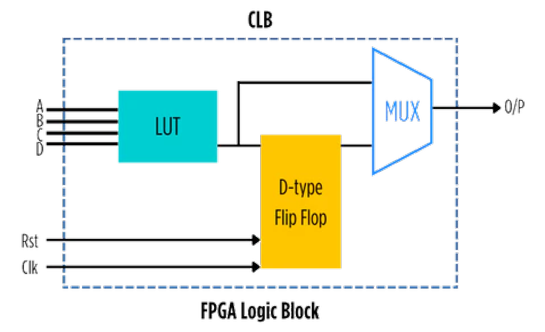
\includegraphics[width=\textwidth]{Figures/fpga_CLB.pdf}
%         \end{figure}
%     \end{columns}
% \end{frame}

\section{Design Flow}

\subsection{Successive Refinement}
\begin{frame}{Gajski-Kuhn chart}{\insertsection ~- \insertsubsection}
    % Present Y chart and spiral steps
    \begin{columns}[c]
        \column{0.49\textwidth}
        \centering
        % \vspace{1.8cm}
        \begin{figure}
            \centering
            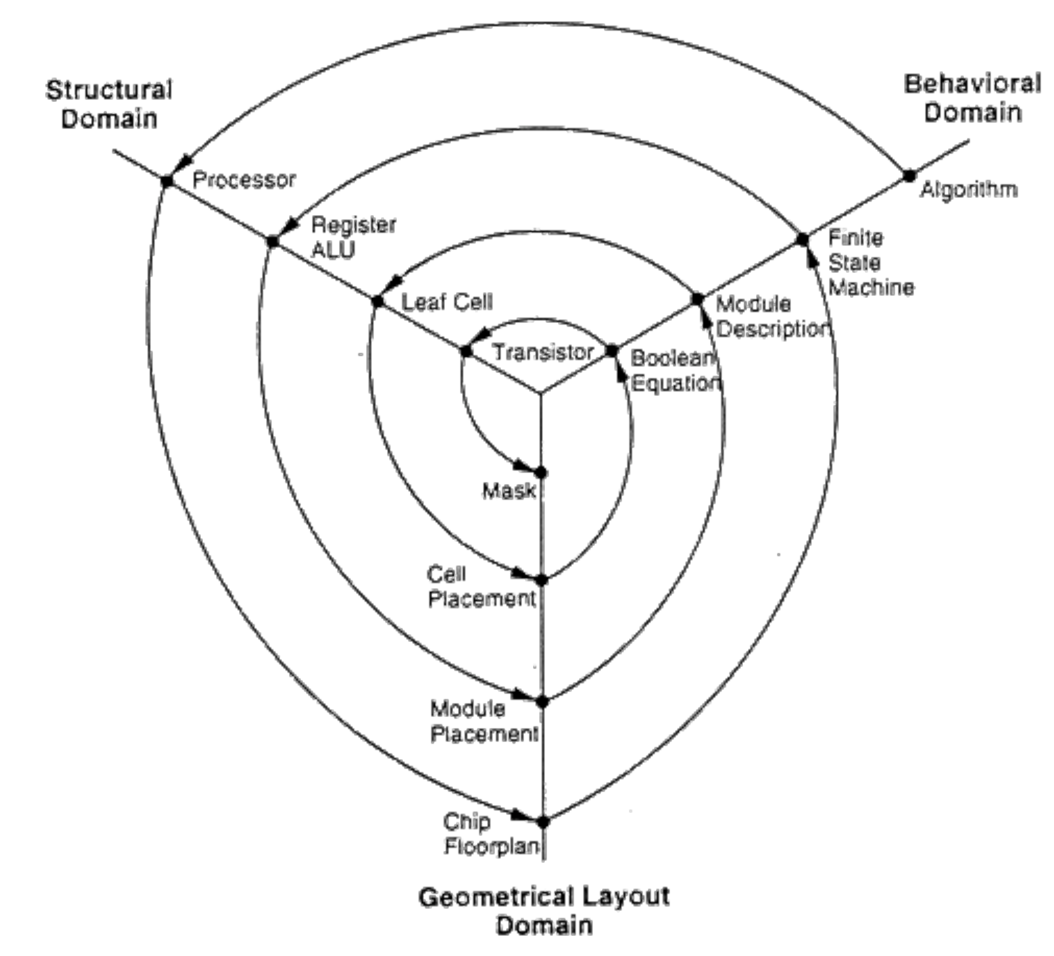
\includegraphics[width=\textwidth]{Figures/y_chart.pdf}
        \end{figure}

        \column{0.49\textwidth}
        \begin{boite1}{Perspectives}
        \begin{itemize}
            \item Behavioral
            \item Structural
            \item Physical/Geometry
        \end{itemize}
        \end{boite1}

        \textbf{Logical synthesis} : from behavioral to structural

        \textbf{Physical synthesis / Layout} : from structural to physical / geometrical

    \end{columns}
\end{frame}

\begin{frame}{Front-End Flow}{\insertsection ~- \insertsubsection}
    % Present HLS and Logic Synthesis
    \begin{columns}[T]
        \column{0.49\textwidth}
        \centering
        \textbf{High Level Synthesis}
        \begin{itemize}
            \item From a system-level description
            \item Produces a Finite State Machine (FSM)
            \item Followed by logical synthesis
        \end{itemize}

        \column{0.49\textwidth}
        \centering
        \textbf{Logical synthesis}
        \begin{itemize}
            \item Takes a RTL description (e.g. FSM) \& technology node
            \item Builds a abstract representation of the logic and maps it to standard cell
            \item Produces a netlist / gate-level circuit
        \end{itemize}
    \end{columns}
\end{frame}

\begin{frame}{Back-End Flow}{\insertsection ~- \insertsubsection}
    % Present Floor plan, Place and Route
    \begin{columns}[c]
        \column{0.39\textwidth}
        Steps :
        \begin{itemize}
            \item Partitioning
            \item Floorplanning
            \item Placement
            \item Global routing
            \item Detailed routing
        \end{itemize}

        \column{0.59\textwidth}
        \begin{figure}
            \centering
            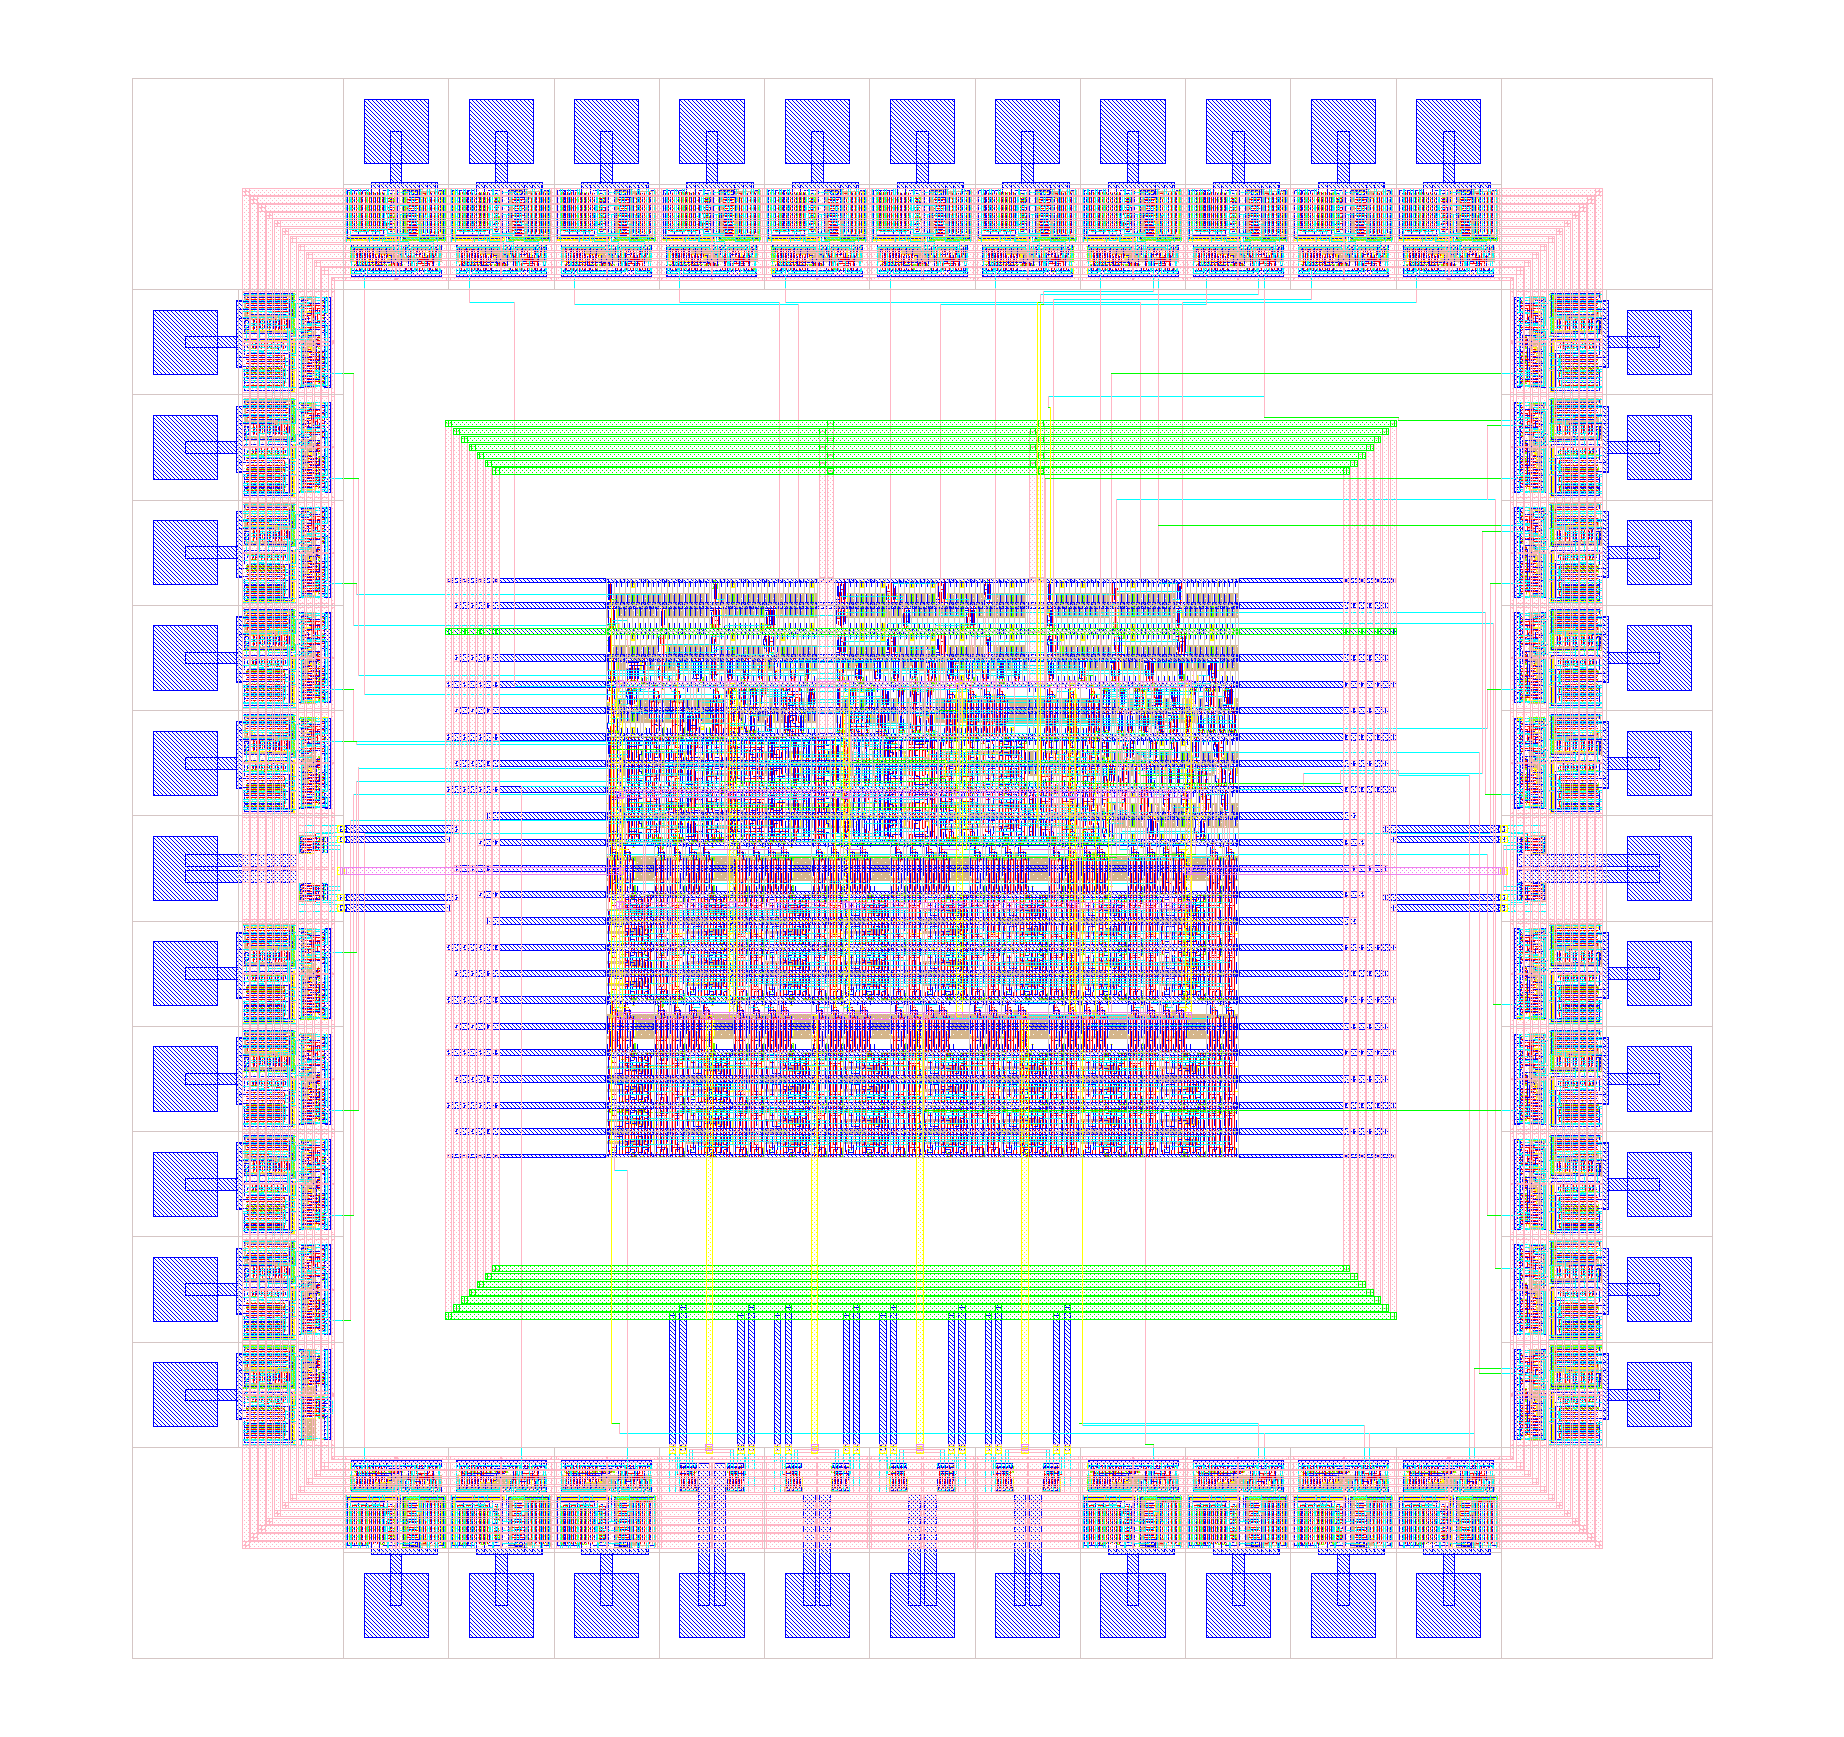
\includegraphics[width=.8\textwidth]{Figures/amd2901_chip_routed.png}
            \caption{Chip layout \cite{noauthor_coriolis_nodate}}
        \end{figure}
    \end{columns}
\end{frame}

\subsection{Verification \& Validation}
\begin{frame}{\insertsubsection}{\insertsection}
    % Present Testbench, golden, different types of simulation
    \begin{columns}[c]
        \column{0.39\textwidth}
        \begin{boite1}{Verification}
            \begin{itemize}
                \item Functional Simulation
                \begin{itemize}
                    \item Behavioral
                    \item Gate-level (Timed)
                    \item Analog
                \end{itemize}
                \item Formal Verification
            \end{itemize}
        \end{boite1}

        \begin{boite}{Validation}
            \begin{itemize}
                \item FPGA (Behavioral)
                \item Static Timing Analysis and Timing Closure
            \end{itemize}
        \end{boite}

        % \begin{boite1}{Formal Verification}
        %     \begin{itemize}
        %         \item
        %     \end{itemize}
        % \end{boite1}

        \column{0.5\textwidth}
        \begin{figure}
            \centering
            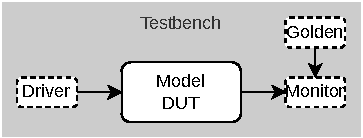
\includegraphics[width=.85\textwidth]{Figures/testbench_model.pdf}
            \caption{Simulated Testbench}
        \end{figure}

        \begin{figure}
            \centering
            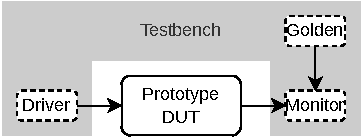
\includegraphics[width=.85\textwidth]{Figures/testbench_hil.pdf}
            \caption{Hardware in the loop}
        \end{figure}
    \end{columns}

\end{frame}

% \begin{frame}{Prototype}{\insertsection ~- \insertsubsection}
%     % Present FPGA and so on
% \end{frame}

% \begin{frame}{Formal Verification}{\insertsection ~- \insertsubsection}
%     % Present KMA stuff
% \end{frame}

\section*{Summary}
\begin{frame}{\insertsection}
 \begin{itemize}
    \item The IC design flow consist of successive refinement accross abstraction layers
    \item Design choices : Flexibility vs Performance, Serial vs Parallel, etc.
    \item CPUs and GPUs are instruction set architectures that execute programs
    \item System on chip are composed of multiple subsystems (IPs)
    \item FPGA are a good platform to prototype hardware designs
 \end{itemize}
\end{frame}

\part{Asynchronous Circuits}
\begin{nonumberframe}
    \vfill
    \centering
    \begin{beamercolorbox}[sep=8pt,center,shadow=false,rounded=true]{title}
    \usebeamerfont{title}Part II - ASYNCHRONOUS CIRCUITS\par%
    \usebeamerfont{subtitle} GUT meeting 13/01/2026
    \end{beamercolorbox}
    \vfill
\end{nonumberframe}

\section{Linear pipeline or digital Fordism}
\begin{frame}{Assembly Line}{\insertsection}
    % Figure Assembly line
\end{frame}

\begin{frame}{Linear Pipeline}{\insertsection}
    % Figure Combinational logic and registers
\end{frame}

\subsection{Concepts}
\begin{frame}{Latency \& Throughput}{\insertsection ~- \insertsubsection}
    % Definition Latency
    % Definition Throughput
\end{frame}

\begin{frame}{Parallelism \& Concurrency}{\insertsection ~- \insertsubsection}
    % Difference between both concepts
    % Introduction of a Fork and a Join
\end{frame}

\section{Clock-driven}
\begin{frame}{Clock Signal}{\insertsection}
    % Global Clock signal
    % Data propagation through global synchronization
\end{frame}
\subsection{Timing Constraints}
\begin{frame}{Linear Pipeline}{\insertsection ~- \insertsubsection}
    % Concept Critical Path
    % Worst case timing
\end{frame}

\begin{frame}{Setup}{\insertsection ~- \insertsubsection}
    % Definition of setup time and chronogram
\end{frame}

\begin{frame}{Hold}{\insertsection ~- \insertsubsection}
    % Definition of hold time and chronogram
\end{frame}

\subsection{Drawbacks}
\begin{frame}{Clock Skew}{\insertsection ~- \insertsubsection}
    % Problem with large clock tree
\end{frame}

\begin{frame}{Clock Domain Crossing}{\insertsection ~- \insertsubsection}
    % Synchronization of datas
    % GALS
\end{frame}

\begin{frame}{Robustness}{\insertsection ~- \insertsubsection}
    % Process variation, Voltage and Temperature
\end{frame}

\section{Event-driven}
\subsection{[TODO] Communication}
\begin{frame}{Local Synchronization}{\insertsection ~- \insertsubsection}
    % Pipeline with local synchronization
\end{frame}

\begin{frame}{Communication Channels}{\insertsection ~- \insertsubsection}
    % Sender, Receiver, Channel, Transaction
\end{frame}

\begin{frame}{Handshakes}{\insertsection ~- \insertsubsection}
    % Level / transition signaling
\end{frame}

\begin{frame}{Control Primitives}{\insertsection ~- \insertsubsection}
    % Uncond and Cond
\end{frame}

\subsection{Transactions at the gate level}
\begin{frame}{Delay Insensitive Circuits}{\insertsection ~- \insertsubsection}
    % Uncond and Cond
\end{frame}

\begin{frame}{State-Holding gates}{\insertsection ~- \insertsubsection}
    % Mueller gate / C-element
\end{frame}

\subsection{Formalism}
\begin{frame}{Petri Nets}{\insertsection ~- \insertsubsection}
    % Token, Place, Transition
\end{frame}

\begin{frame}{Signal Transition Graph}{\insertsection ~- \insertsubsection}
    % 4P Handshake and WCHB controller
\end{frame}

\section{Bundled-Data}
\begin{frame}{Transaction at the pipeline level}{\insertsection ~- \insertsubsection}
    % Control path, data path
    % matched delay
\end{frame}

\subsection{Timing Constraints}
\begin{frame}{Setup \& Hold}{\insertsection ~- \insertsubsection}
    % Relative Timing Constraints
    % Delay equations
\end{frame}

\begin{frame}{Local Clock Sets}{\insertsection ~- \insertsubsection}
    % Static Timing Analysis
    % During logical synthesis and PnR
\end{frame}

\section*{Summary}
\begin{frame}{\insertsection}

\end{frame}

\appendix
\begingroup
  \addtocounter{part}{-1}
    \part{Appendices}
    \AtBeginSection[]{
        \begin{nonumberframe}{Table of contents}
            \tableofcontents[currentsection,part={3}]
        \end{nonumberframe}
    }

    \section{References}
    \begin{frame}[allowframebreaks]{\insertsection}
      \printbibliography
    \end{frame}

    % \section{Oligopoly problem in VLSI}
\begin{frame}{Problematic}{\insertsection}
    % Few EDA, PDK, Foundries
\end{frame}

\begin{frame}{OPENROAD}{\insertsection}
    % Present the project and Skywater 130, Yosys ABC, ACT etc
\end{frame}

\begin{frame}{CHIPS}{\insertsection}
    % Present the project Coriolis, IHP PDK etc
\end{frame}

\section{Metastability \& Arbiters}
\begin{frame}{Metastability in Clock Domain Crossing}{\insertsection}
    % Why two stage of registers
\end{frame}

\begin{frame}{Metastability in Arbiters}{\insertsection}
    % Mutex element
    % Physical properties to resolve metastability
\end{frame}

\section{Properties of Petri Nets \& STG}
\begin{frame}{Petri Nets}{\insertsection}
    % Present Dead lock, Safety, Liveliness
\end{frame}
\begin{frame}{Signal Transition Graph}{\insertsection}
    % Present decomposition of a WCHB controller
\end{frame}
% \begin{frame}{Workcraft}{\insertsection}
%     % Present workcraft tool for simulation and analysis
% \end{frame}

\section{Families of Bundled-Data circuits}
\begin{frame}{Occupancy \& Static Spread}{\insertsection}
    % Present tokens in a pipeline
\end{frame}
\begin{frame}{Coupling}{\insertsection}
    % Present the relation between coupling and static spread, the interdependence in data
\end{frame}
\begin{frame}{Capture}{\insertsection}
    % Present the difference between early and late capture, and its impact on RTZ
\end{frame}
\begin{frame}{Latched Controller}{\insertsection}
    % Click Mousetrap
\end{frame}
\endgroup
\end{document}
